\newcommand{\CLASSINPUTbaselinestretch}{1.0} % baselinestretch
\newcommand{\CLASSINPUTinnersidemargin}{0.75in} % inner side margin
\newcommand{\CLASSINPUToutersidemargin}{0.75in} % outer side margin
\newcommand{\CLASSINPUTtoptextmargin}{0.75in}   % top text margin
\newcommand{\CLASSINPUTbottomtextmargin}{0.75in}% bottom text margin

\newcommand{\revised}[1]{{\color{blue}#1}}

\documentclass[conference]{IEEEtran}

\IEEEoverridecommandlockouts % precisa para usar o \thanks{}
% *** CITATION PACKAGES ***
%
\usepackage{cite}
\usepackage{flushend}
\usepackage{xcolor}
\usepackage[pdftex]{graphicx}

\usepackage[utf8]{inputenc}


% *** MATH PACKAGES ***
%
%\usepackage[cmex10]{amsmath}
\usepackage{amsmath}
\usepackage{amssymb}

% *** SPECIALIZED LIST PACKAGES ***
%
\usepackage{algorithm}
\usepackage{algorithmic}

% *** ALIGNMENT PACKAGES ***
%
\usepackage{array}
\usepackage{multirow}

% *** SUBFIGURE PACKAGES ***
\usepackage[tight,footnotesize]{subfigure}

% *** PDF, URL AND HYPERLINK PACKAGES ***
%
%\usepackage[bookmarks=false]{hyperref}
\usepackage{url}

% correct bad hyphenation here
\hyphenation{rep-re-sen-ta-tion fe-de-ral}


\begin{document}
%
% paper title
% can use linebreaks \\ within to get better formatting as desired
\title{\vspace{0.25in}Avaliação estatística sobre seleção de características para categorização de texto}


% author names and affiliations
% use a multiple column layout for up to three different
% affiliations

\author{\IEEEauthorblockN{
		Rog\'{e}rio C. P. Fragoso\IEEEauthorrefmark{1}, 
		Lucas F. Melo\IEEEauthorrefmark{1},
		Saulo C. R. P. Sobrinho\IEEEauthorrefmark{1}
}
\IEEEauthorblockA{Universidade Federal de Pernambuco (UFPE), Centro de Inform\'{a}tica (CIn)\\
Av. Jornalista Anibal Fernandes s/n, Cidade Universit\'{a}ria 50740-560, Recife, PE, Brazil\\
rcpf@cin.ufpe.br, lfm2@cin.ufpe.br, scrps@cin.ufpe.br \\}}
%\IEEEauthorrefmark{1}Telephone: +55 81 2126-8430 Ext.4346 Fax: +55 81 2126-8438}}

% make the title area
\maketitle

\begin{abstract}
	%\boldmath
\textcolor{red}{ESCREVER RESUMO}
\end{abstract}

\IEEEpeerreviewmaketitle

% Formato descrito na página da disciplina. Lá ela diz que a presença destas seções é mandatória. 
% (Acho que a gente não precisa organizar nesse formato exatamente, mas precisamos garantir que cada item esteja presente)

%•       Passo 1 – Justificativa: De início, explicitam-se os motivos que justificam a pesquisa, determinando-se e delimitando-se o problema, o qual deve estar formulado de maneira clara e precisa.
%•       Passo 2 - Fundamentação teórica: Descreve-se  o relacionamento do problema com a teoria que será utilizada na pesquisa.
%•       Passo 3 - Objetivo da pesquisa: Os objetivos devem ser retirados diretamente dos problemas levantados no Passo 2. Define-se o que se pretende alcançar com a realização do trabalho.
%•       Passo 4 - Especificação da amostra: Deve-se determinar a área de execução da pesquisa, a população a ser investigada, o tipo de amostra e a determinação do seu tamanho, bem como o tipo de amostragem a ser utilizado. Define-se as variáveis envolvidas.
%•       Passo 5– Análise exploratória: Fazer um estudo descritivo dos dados (gráficos e medidas).  Verificar normalidade dos dados e potenciais pontos aberrantes.
%•       Passo 6– Metodologia (Formulação das hipóteses): Estabelecem-se as hipóteses que serão formuladas, as quais devem ser claras e precisas. Define-se o problema estatisticamente, decidindo-se que informação estatística é realmente necessária e qual método que será aplicado.   
%•       Passo 7 - Análise dos resultados: Passa-se ao tratamento dos dados por intermédio dos testes estatísticos, os quais dependem das hipóteses que serão testadas. Nesse tópico, é exigido que sejam aplicados testes de hipóteses paramétricos e/ou não paramétricos. Testes de duas amostras são exigidos, quando comparando abordagens.

\section{Introdução}
\label{sec:intro}

Algoritmos são sequências de instruções bem definidas, porém suas implementações podem apresentar comportamentos difíceis de serem previstos.
Seja pelo uso de geração de números pseudo-aleatórios que geram um comportamento não determinístico inerente ao código, ou pelo uso de linguagens de alto nível cuja tradução para linguagem de máquina passa por otimizações e diferentes interações com a arquitetura de destino na qual o algoritmo é executado.
Sendo assim, a performance de algoritmos de computação em geral é não-determinística e, ao analisar comparativamente o desempenho destes algoritmos, é necessário levar em consideração que estamos diante de uma amostra aleatória que representa estas performances.

Este trabalho realiza uma comparação entre algoritmos de categorização de texto, mostrando como determinar e aplicar testes estatísticos adequados para este cenário.

\subsection{Fundamentação teórica}
%Seguindo o modelo sugerido no site, essa seção é obrigatória.
\textcolor{red}{Nesta seção, apresentar o problema de seleção de características, categorização de textos e os conceitos básicos necessários para o entendimento do trabalho.}

Esta seção apresentou conceitos básicos de categorização de textos e seleção de características. 
O restante do trabalho é organizado como segue: 
A Seção \ref{sec:objetivo} apresenta o objetivo do presente trabalho. 
Na Seção \ref{sec:exp} são detalhadas as configurações dos experimentos, incluindo descrição da base de dados, os algoritmos de interesse e as hipóteses a serem verificadas sobre os dados. 
A Seção \ref{sec:analise} demonstra os procedimentos estatísticos realizados no trabalho.
Finalmente, a Seção \ref{sec:conclusao} apresenta as conclusões do trabalho.

\section{Objetivo}
\label{sec:objetivo}

O objetivo do presente trabalho é avaliar e comparar o desempenho de quatro métodos de seleção de características usados em categorização de texto.
Esta análise comparativa permite determinar se os algoritmos possuem desempenhos significativamente diferentes e, em caso positivo, determinar quais deles se destacam dos demais.

%Para tanto, executamos análises estatísticas para avaliar a aderência dos dados amostrais a uma distribuição normal.
%Posteriormente, aplicamos testes de hipóteses adequados para, efetivamente, comparar os desempenho dos métodos.

\section{Experimentos}
\label{sec:exp}

Esta seção descreve as configurações dos experimentos realizados para gerar o conjunto de dados sobre o qual a análise será realizada.

\subsection{Base de dados}
\label{sec:bd}

Neste trabalho, a base de dados \textit{Reuters 10} foi utilizada.
Esta base de dados é um subconjunto da coleção \textit{Reuters-21578}~\footnote{Disponível em http://disi.unitn.it/moschitti/corpora.htm.}, que é uma das bases mais utilizadas em trabalhos de categorização de texto.
A base é composta por documentos coletados do \textit{Reuters newswire} de 1987 e apresenta 135 categorias.
Entretanto, neste trabalho foi adotado um subconjunto composto pelas 10 maiores categorias da base.
O subconjunto \textit{Reuters 10} contém 9.980 documentos e seu vocabulário abarca 10.987 termos.
A base de dados \textit{Reuters 10} também é bastante utilizada em trabalhos de categorização de texto~\cite{chang2008multilabel,chen2009feature,yang2011new}. 

A distribuição dos documentos é bastante desbalanceada, apresentando categorias representando desde 2,3\% até 39\% do tamanho total da base. 
Nesta base foram aplicados os seguintes procedimentos de pré-processamento:
remoção de termos com duas ou menos letras, remoção de \textit{stopwords} e \textit{stemming}, com o algoritmo \textit{Iterated Lovins
Stemmer}~\cite{lovins1968development}.

Vale salientar que, para os propósitos da disciplina, o uso de repositórios como base para análise não é encorajado. Contudo, a análise comparativa deste trabalho será realizada sobre o desempenho dos algoritmos, tendo a base citada como entrada, e não sobre características da base em si.

\subsection{Metodologia}
\label{sec:metodologia}

Conforme mencionado na Seção \ref{sec:objetivo}, estamos interessados na comparação de desempenho de algoritmos de seleção de características para categorização de texto.
Neste trabalho, a comparação é realizada entre os algoritmos \textit{Maximum Features per Document} (MFD), \textit{Maximum Features per Document-Reduced} (MFDR), \textit{Category-dependent Maximum Features per Document-Reduced} (cMFDR) e \textit{Automatic Feature Subsets Analyzer} (ASFA). A avaliação dos desempenhos dos métodos foi realizada utilizando o algoritmo classificador \textit{Na\"ive Bayes Multinomial}~\cite{mccallum1998comparison} e a base de dados \textit{Reuters 10}. Deste modo, a base de dados é pre-processada para cada um dos quatro algoritmos de seleção de carcaterísticas, gerando, assim, quatro versões da base original. Em seguida, o classificador \textit{Na\"ive Bayes Multinomial} é  treinado e testado com cada uma destas quatro versões.

A validação cruzada estratificada foi utilizada como método para estimativa de desempenho.
Esta técnica é adotada para avaliar a capacidade de generalização de um modelo a partir de um conjunto de dados.
Neste trabalho, utilizou-se a variação validação cruzada estratificada com \emph{10 folds}, na qual a base de dados $\mathcal{D}$ é particionada em 10 subconjuntos (\emph{folds}), de tamanhos semelhantes, mantendo a proporção de documentos por categorias equivalente à proporção encontrada no conjunto original. Então, são construídos 10 classificadores, cada um utilizando uma parcela dos \emph{folds} para treinamento e outra parcela para realizar o teste do mesmo, de modo a gerar diferentes combinações dos \emph{folds}.
A avaliação final é dada pela média das medidas obtidas em cada uma das 10 execuções~\cite{kohavi1995study}.
Nos experimentos realizados com os métodos MFD, MFDR e cMFDR, nove partições foram utilizadas para treinamento e uma partição foi utilizada para teste.
O método AFSA requer uma porção dos dados para configuração de seus parâmetreos. Assim, os experimentos executados com AFSA utilizaram oito partições para treinamento, uma para configuração de parâmetros/validação e uma para teste.

Assim, temos dez medidas de desempenho para cada um dos quatro métodos de seleção de características avaliados.
Estes dados de desempenho correspondem às entradas para as análises estatísticas realizadas neste trabalho.

A medida de desempenho utilizada nos experimentos foi \textit{Micro-F1}.
Seu cálculo é dado pela Eq.~\ref{eq:micro_f1}.

\begin{equation}
\operatorname{\mathcal{F}{1} = \frac{2 x \mathcal{P} x \mathcal{R}}{\mathcal{P} + \mathcal{R}}},
\label{eq:micro_f1}
\end{equation}

\noindent onde $\mathcal{P}$ é uma medida de precisão e $\mathcal{R}$ é uma medida de cobertura~\cite{chang2008multilabel}. As fórmulas para calcular a precisão $\mathcal{P}$ e a cobertura $\mathcal{R}$ são exibidas a seguir.

\begin{equation}
\operatorname{\mathcal{P}} = \frac{\sum_{j=1}^{C}TP_j}{\sum_{j=1}^{C}(TP_j + FP_j)}
\label{eq:precision}
\end{equation}

\begin{equation}
\operatorname{\mathcal{R}} = \frac{\sum_{j=1}^{C}TP_j}{\sum_{j=1}^{C}(TP_j + FN_j)}
\label{eq:recall}
\end{equation}

$TP_j$ é a quantidade de instâncias corretamente rotuladas como pertencentes à categoria $c_j$; $FP_j$ é a quantidade de instâncias incorretamente rotuladas como pertencentes à categoria $c_j$; e $FN_j$ é a quantidade de instâncias incorretamente rotuladas como não pertencentes à categoria $c_j$. 

\section{Análise estatística}
\label{sec:analise}

\subsection{Estatística descritiva}

Uma boa prática ao iniciar uma análise de conjunto de dados, a qual é sugerida por muitos autores, é o uso de técnicas de estatística descritiva para se obter intuições iniciais acerca do conjunto de interesse \cite{montgomery2010applied}.

Para se ter uma indicação sobre os tipos de testes que podem ser executados sobre os dados, é interessante verificar se as distribuições que geram os dados aparentam normalidade.
A suposição de normalidade é útil pois, se esta for plausível, podemos aplicar testes paramétricos sobre os dados.
Testes paramétricos possuem maior poder estatístico do que seus equivalentes não-paramétricos, o que nos permite extrair conclusões mais fortes.

Para verificar a normalidade, começamos utilizando ferramentas visuais.
Histogramas permitem visualizar a distribuição das amostras e consequentemente intuir sobre a distribuição da população geradora.
As Figuras~\ref{fig:hist_afsa} a~\ref{fig:hist_mfd} apresentam os histogramas das amostras.

\begin{figure}[h]
	\centering
	\includegraphics[width=\linewidth]{img/bluehist_afsa.pdf}
	\caption{Histograma dos ... do algoritmo AFSA (10 amostras)}
	\label{fig:hist_afsa}
\end{figure}

\begin{figure}[h]
	\centering
	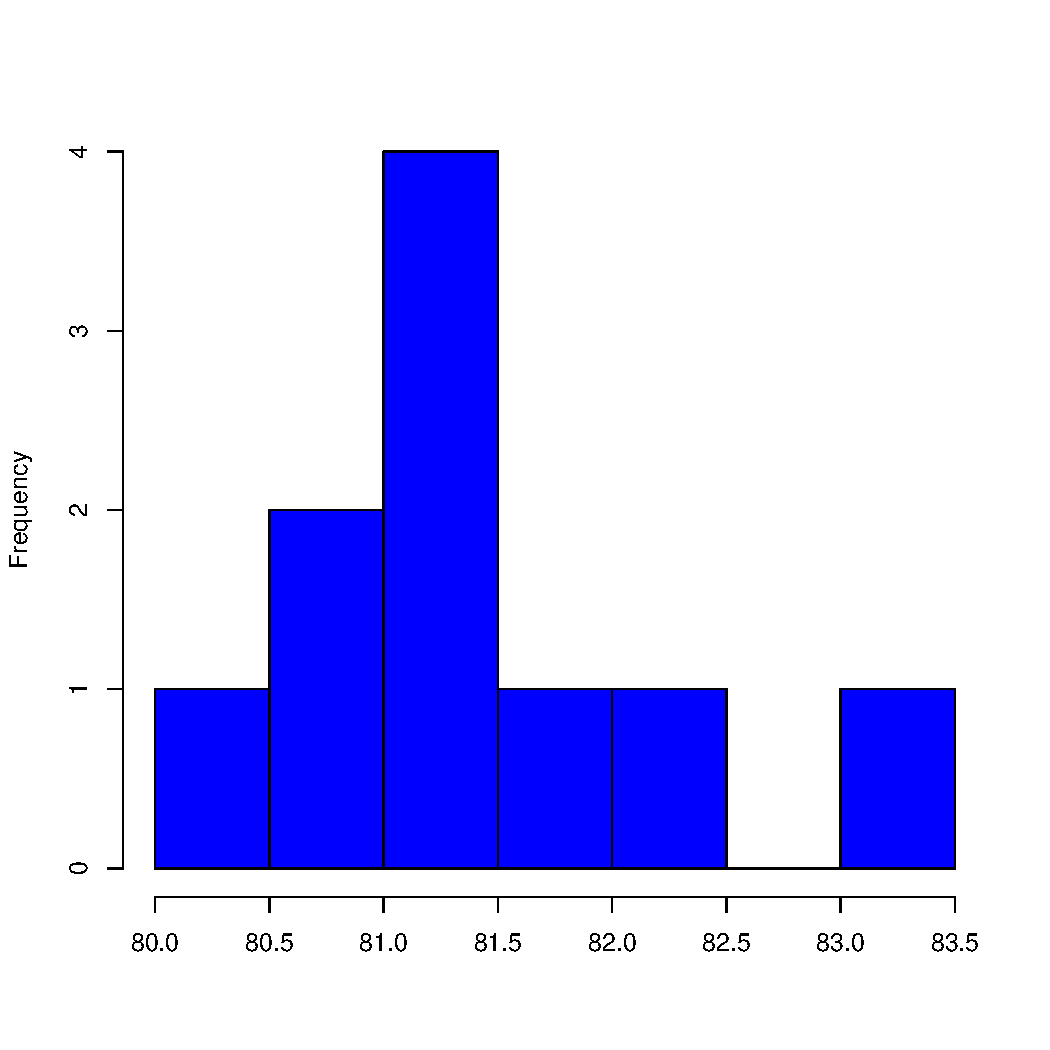
\includegraphics[width=\linewidth]{img/bluehist_cmfdr.pdf}
	\caption{\textcolor{red}{Escrever uma descrição}.}
	\label{fig:hist_cmfdr}
\end{figure}

\begin{figure}[h]
	\centering
	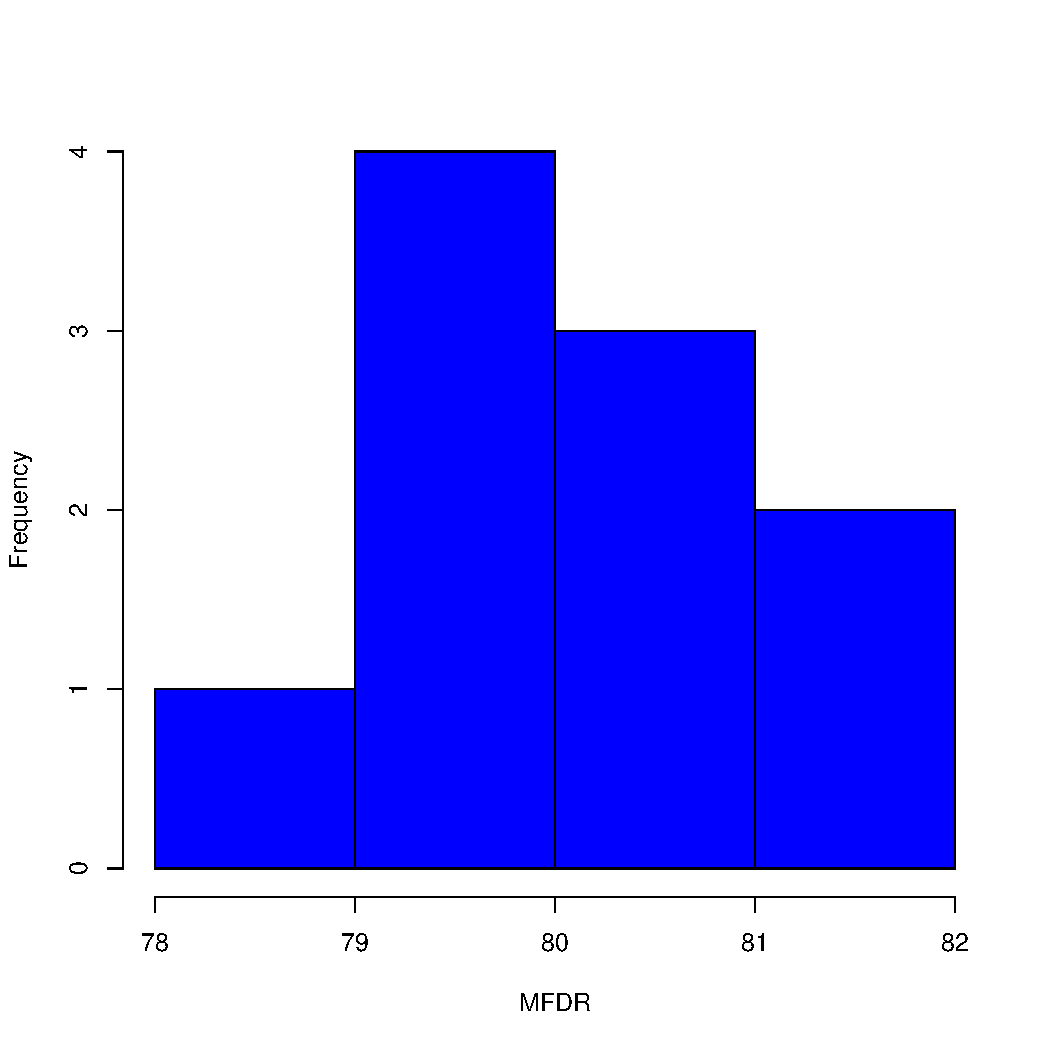
\includegraphics[width=\linewidth]{img/bluehist_mfdr.pdf}
	\caption{\textcolor{red}{Escrever uma descrição}.}
	\label{fig:hist_mfdr}
\end{figure}

\begin{figure}[h]
	\centering
	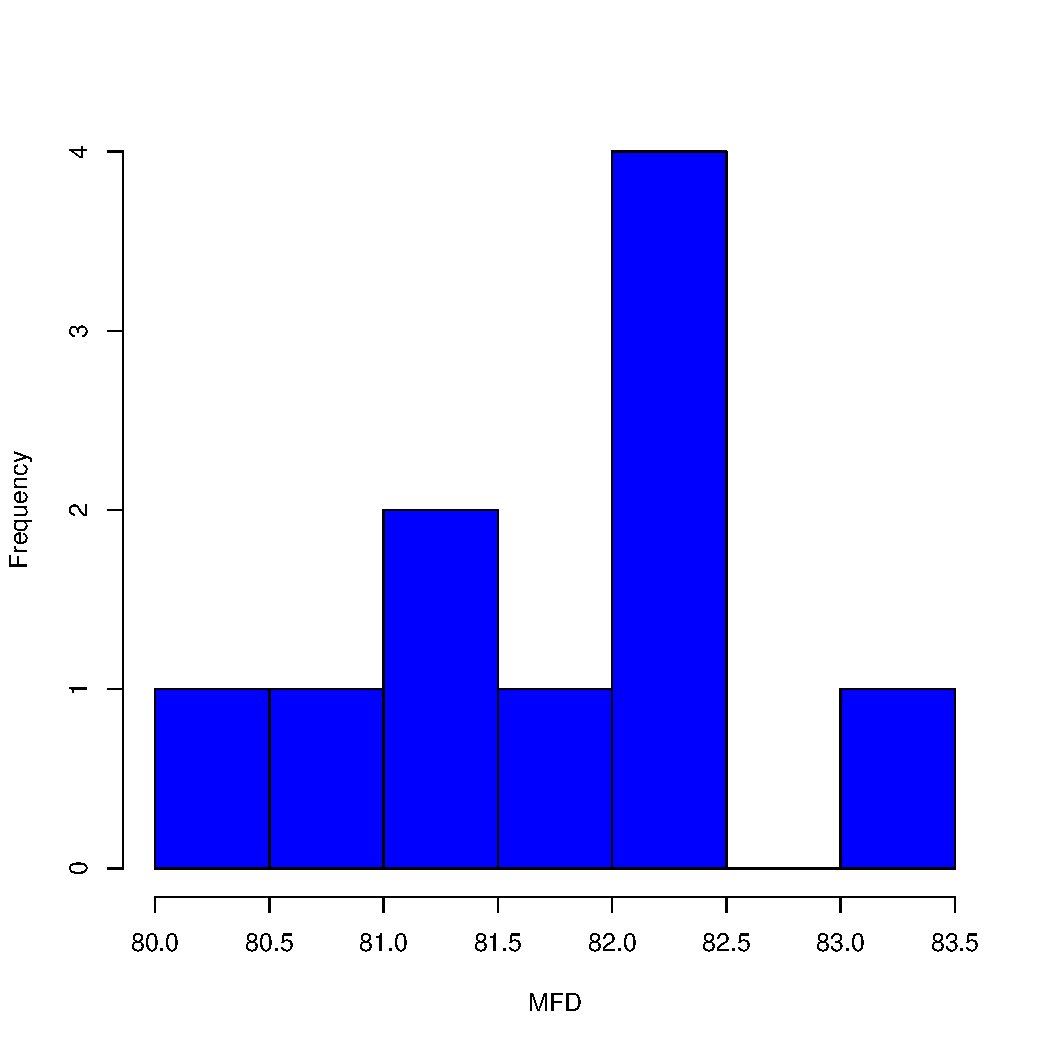
\includegraphics[width=\linewidth]{img/bluehist_mfd.pdf}
	\caption{\textcolor{red}{Escrever uma descrição}.}
	\label{fig:hist_mfd}
\end{figure}

A julgar pelos histogramas apresentados, não temos motivo para acreditar que tais amostras sejam provenientes de distribuições normais.
Para juntar mais evidências, continuaremos a análise com mais recursos.

Outra ferramenta visual útil é o \textcolor{red}{plot de probabilidade normal} ou \textit{normplots}, que permite verificar o quão bem os dados podem ser ajustados por uma distribuição normal.
Quando os dados são plotados dessa forma, uma linha reta indica uma distribuição normal ideal, sendo essa linha plotada para ser usada como referência.
Num cenário real, devido à presença de ruídos, não se espera que os dados se adequem perfeitamente à reta, porém se espera que, se os dados forem provenientes de uma distribuição normal, estes sejam bem aproximados pela reta de referência e estejam próximos a ela.
As Figuras \ref{} a \ref{} mostram os normplots de cada distribuição.

\begin{figure}[h]
	\centering
	\includegraphics[width=\linewidth]{img/bluenorm_afsa.pdf}
	\caption{Normplot dos ... do algoritmo AFSA (10 amostras)}
	\label{fig:hist_afsa}
\end{figure}

\begin{figure}[h]
	\centering
	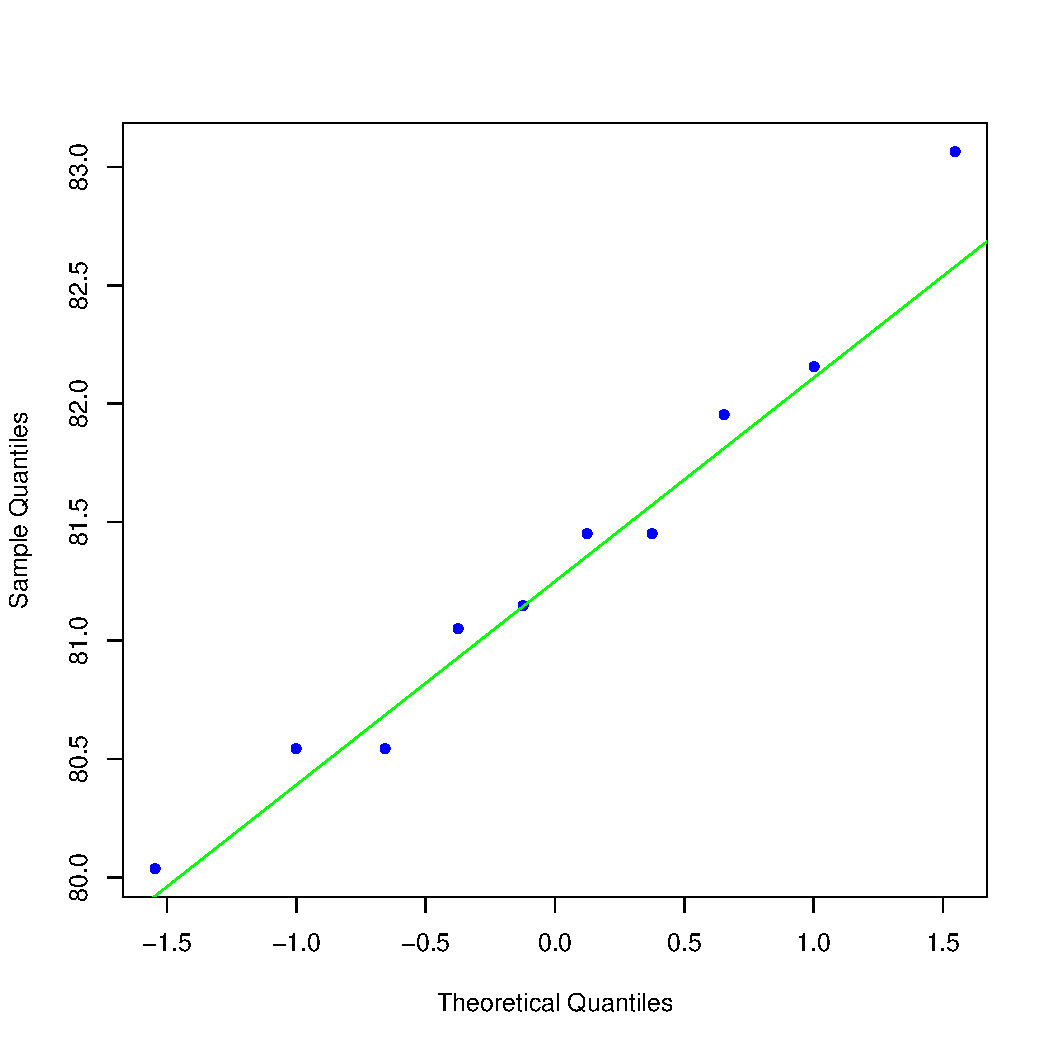
\includegraphics[width=\linewidth]{img/bluenorm_cmfdr.pdf}
	\caption{\textcolor{red}{Escrever uma descrição}.}
	\label{fig:hist_cmfdr}
\end{figure}

\begin{figure}[h]
	\centering
	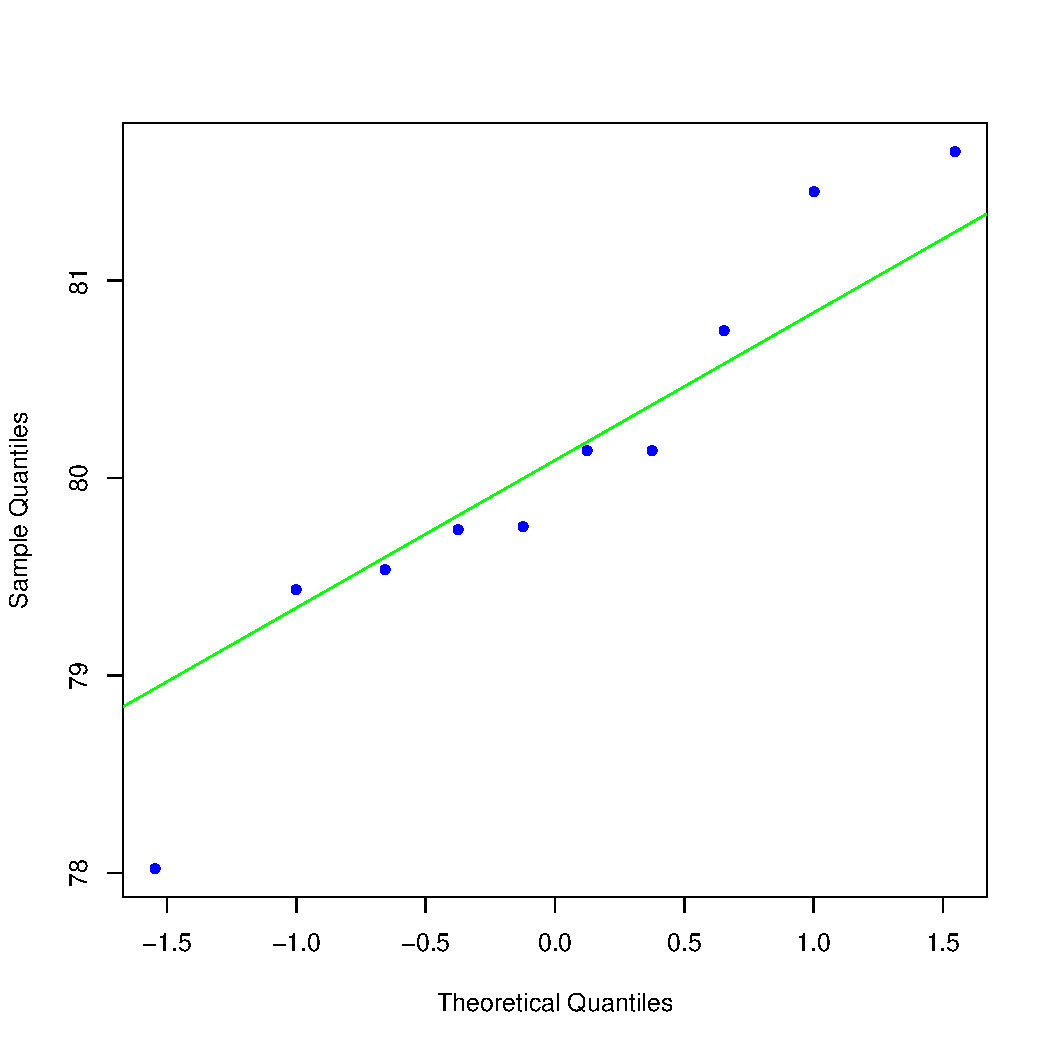
\includegraphics[width=\linewidth]{img/bluenorm_mfdr.pdf}
	\caption{\textcolor{red}{Escrever uma descrição}.}
	\label{fig:hist_mfdr}
\end{figure}

\begin{figure}[h]
	\centering
	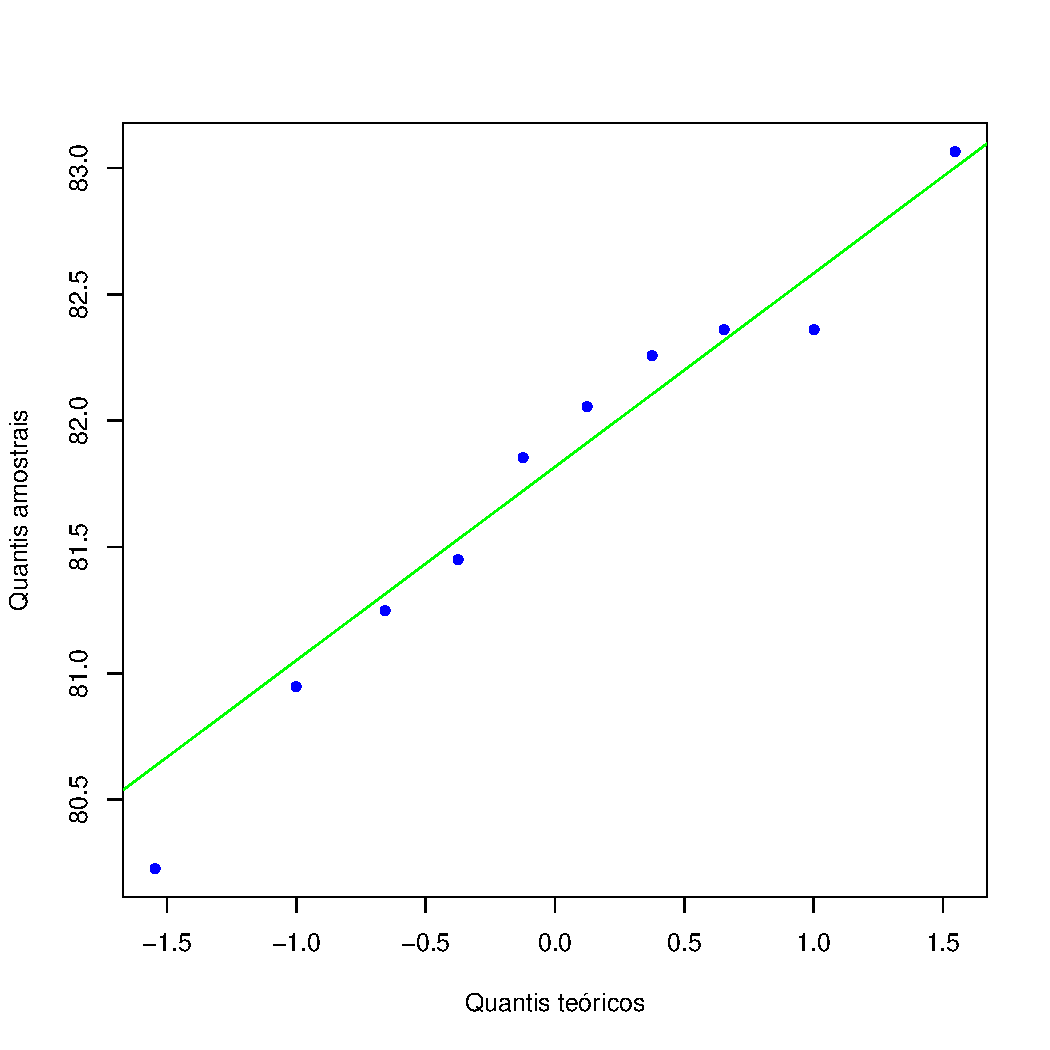
\includegraphics[width=\linewidth]{img/bluenorm_mfd.pdf}
	\caption{\textcolor{red}{Escrever uma descrição}.}
	\label{fig:hist_mfd}
\end{figure}

\textcolor{red}{ISSUE: Os pontos não aparecem quando o latex importa o pdf Oo [Lucas: os pontos aparecem pra mim; além disso, minha impressão é que, se tivéssemos mais dados, os pontos se aproximariam da reta. Será que podemos afirmar que não é normal?]}
Podemos observar que os dados não se aproximam tão bem de uma linha reta.

Por último ainda recorremos aos plot de caixa para verificar em particular a simetria dos dados. ...

Para confirmar nossa intuição de que as amostras não são normalmente distribuídas, recorremos a testes de hipótese utilizados para verificação de normalidade.
Os testes usados foram o de Shapiro-Wilk \cite{shapiro1965analysis} e ...	

\textcolor{red}{As amostras pequenas se mostraram um fator limitante da análise...}

\begin{table}[h]
	\centering
	\caption{Estatística descritiva}
	\label{tab:est_descr}
	\begin{tabular}{cccc}
		Método    & Média  & Mediana & Desv. Padrão  \\
		\hline
		AFSA&		81.05262 	& 80.9594 	& 0.9634384 \\
		cMFDR&      81.39266 	& 81.38469 	& 1.027409 \\
		MFDR& 		79.03808 	& 79.05812 	& 1.119577 \\
		MFD&     	81.93872 	& 81.91752 	& 1.029598 \\
		\hline
	\end{tabular}
\end{table}

\textcolor{red}{FALAR SOBRE OS RESULTADOS
Quais aparentam ser normais (média aprox. igual à mediana)
}


A Figura~\ref{fig:boxplot} apresenta uma.....

\begin{figure}[h]
	\centering
	\includegraphics[width=\linewidth]{img/boxplot.pdf}
	\caption{\textcolor{red}{Escrever uma descrição}.}
	\label{fig:boxplot}
\end{figure}



\textcolor{red}{FAZER UMA CONCLUSÃO DA SEÇÃO
Falar das impressões sobre a normalidade dos dados com bases nos histogramas, boxplot e medidas estatísticas.......}

\subsection{Testes de aderência}
Dado que os resultados visuais não foram conclusivos o suficiente, especialmente pelo fato de os conjuntos de dados serem pequenos, se torna interessante realizar um teste para verificação da normalidade dos dados...

\textcolor{red}{Escrever uma motivação para o uso dos testes de aderência e uma breve explicação de como funcionam}

A Tabela~\ref{tab:aderencia} exibe os resultados dos testes Shapiro-Wilk e Kolmogrov-Smirnov para os quatro métodos.

\begin{table}[h]
	\centering
	\caption{Resultados dos testes de aderência}
	\label{tab:aderencia}
	\begin{tabular}{c|ccc}
		\hline
		& \multicolumn{2}{c}{p-value}      \\
		\cline{2-3}
		& Shapiro-Wilk & Kolmogrov-Smirnov \\
		\hline
		AFSA  & 0.2353       & 0.1818            \\
		cMFDR & 0.3107       & 0.1818            \\
		MFDR  & 0.6773       & 0.1818            \\
		MFD   & 0.3597       &  0.1818               \\
		\hline
	\end{tabular}
\end{table}

\textcolor{red}{Escrever sobre os resultados do test Shapiro-Wilk}

\textcolor{red}{Escrever sobre os resultados do test Kolmogrov-Smirnov}

\subsection{Testes de hipóteses}

\textcolor{red}{Ainda não executei os testes de hipóteses}

\section{Conclusão}
\label{sec:conclusao}

\textcolor{red}{Escrever conclusão}



\bibliographystyle{IEEEtran}
% argument is your BibTeX string definitions and bibliography database(s)
% \bibliography{IEEEabrv,../bib/paper}
\bibliography{bb}

\end{document}
